\documentclass[11pt]{article}

\usepackage[margin=0.75in]{geometry}
\usepackage{indentfirst}
\usepackage{graphicx}
\usepackage{hyperref}
\usepackage{caption}
\usepackage{amsmath}
\usepackage{float}

\bibliographystyle{siam}

\title{Examining Self-Control Through the BART Study}
\author{
  Chen, Kent\\
  \texttt{kentschen}
  \and
  Lee, Rachel\\
  \texttt{reychil}
  \and
  LeRoy, Benjamin\\
  \texttt{benjaminleroy}
  \and
  Liang, Jane\\
  \texttt{janewliang}
  \and
  Udagawa, Hiroto\\
  \texttt{hiroto-udagawa}
}



\begin{document}
\maketitle

\abstract{% tex file for abstract
\par Self-control is an interesting field of behavioral research with broad 
implications for our day-to-day experiences. Being able to appropriately 
regulate and check our impulses and reactions to various everyday stimuli 
is necessary for maintaining health and high-functionality in society. 
Thus, relating a subject’s ability to control risky behavior to an area 
of the brain has been the focus of many studies. One approach to 
capturing these neurological facets is to use functional magnetic resonance 
imaging (fMRI). Our goal is to identify active regions of the brain using 
fMRI data from a Balloon Analogue Risk Task (BART) study described in 
Cohen's \textit{The Development and Generality of Self-Control} 
\cite{CohenSelfControl}. When possible and logically sound, we will attempt 
to reproduce the data preprocessing and analysis outlined in the paper. 
However, many of our approaches deviate considerably from the methods 
used by Cohen, either out of necessity from our lack of pre-packaged 
software or when we were inspired explore other directions. Ultimately, we 
will compare the active regions identified by our analysis with those 
detected by the Cohen's paper. 
}

\section{Introduction} \label{introduction}
	% tex file for introduction
\par This paper, \textit{The Development and Generality of Self-Control} \cite{CohenSelfControl},  and its associated fMRI studies are concerned with the relationship between impaired and normal self control as well as the similarities and differences across the brain relating to self-control. The entire paper explores multiple studies (of multiple study types), but we will just focus on the third and final study, which compares four different types of self control among healthy adults to see if they are related to each other. Very little relationship was found between these behavioral tasks, in contrast to the vast majority of existing literature, which argues for a unified notion of self-control, which is why we have decided to narrow the data analysis approaches to just the BART study. The BART study primarily focused on the inflation/deflation of a balloon that could pop; the fMRI scans show blood flow to the brain in an attempt to reveal control over risk-taking behavior while subjects participate in this particular study.
\par The rest of this report will go further in detail on the processes that we have tried to mimic from the original analysis of the data, but here is a brief overview of the work we have accomplished so far. We have looked into spatial smoothing of the data on the voxels of the brain. After realizing that there are many factors that could contribute to noise in the data, we decided it would be beneficial to look into smoothing modules in Python that could handle n-dimensional datasets to clarify which voxels are more important than other voxels. After obtaining convolved time courses for each subject, we turned to fitting simple and multiple linear regression models to each subject. Since examining the behavior of blood flow in the voxels over time was of such great interest, we also considered modeling the behavior as a time series using an autoregressive integrated moving average (ARIMA). 


\section{Data} \label{data}

	% tex file for data
\par \indent The Balloon Analogue Risk Task (BART) measures risk-taking 
behavior by presenting participants with a computerized balloon. The 
participant can earn money incrementally by pumping up the balloon, but after 
an unknown threshold, the balloon will explode. At any time, the participant 
elect to cash out his or her earnings, but doing so eliminates the potential to 
gain additional money through pumps. If the balloon explodes, the participant 
loses all of the money for the trial. For this study, BART and fMRI data for 24 
subjects was collected. The mean age of the subjects was 20.8, and ten of the 
subjects were female. Four behavioral variables were recorded for each subject: 
the average number of pumps for each balloon, the average amount of money 
earned across runs, the number of exploded balloons, and the number of trials. 
There were also three model conditions: events for inflating the balloon 
(excluding the very last inflation of each trial), the last inflation before an 
explosion, and the event of cashing out (the balloon explosion was not included 
as an event). Of interest for our work is the blood-oxygen-level dependent 
(BOLD) imaging data recorded for each subject during the course of task. Each 
subject's BOLD data was recorded as 64 by 64 image matrices in 34 slices, with 
a variable number of time points. 

	
\section{Methods} \label{methods}
	\subsection{Smoothing}
	
		% tex file for smoothing
\par \indent Due to the random nature of human subjects and their movements, a certain extent of smoothing must be performed on the spatial dataset so that the ‘noisy’ data can be cast off from the data that represent significant changes in blood flow in the brain. By doing so, researchers and anyone else investigating the data will be able to distinguish between non-brain scans versus actual brain scans. Each voxel of the brain is represented on a measure of blood flow intensity, and so a series of steps must be taken so that it is correctly convolved to most closely and accurately depict what was happening at a certain point in the brain at a certain time. After researching quite extensively, we decided to use a convolution involving a Gaussian kernel in order to smooth the three dimensional data. Originally, we were going to try and write a smoothing function from scratch, by implementing a rudimentary rudimentary average-over-neighbors method. However, discussions with mentors lead us to the scipy module called \texttt{ndimage.filters} that has a function that performs a Gaussian filter on n-dimensional data. This was exactly what we needed so rather than reinventing the wheel, we will be smoothing the data with this module.

	\subsection{Convolution and Time Correction of Hemodyamic Response}

		% tex file for convolution
\subsubsection{Convolution}
\par \indent Our study is structured around event-related neurological 
stimulus, rather than block stimulus, as was the case of the data used in 
class examples. So, we could not repurpose the class approach for 
representing the hemodynamic response to our analysis. 

\par It is assumed that there is a relationship between the hemodynamic 
response to the neurological stimuli. Further, there is the assumption that 
a single stimulus generates a delayed hemodynamic response that mirrors a 
double-gamma function, and that multiple stimuli have an additive nature, as 
defined below: 

\begin{equation} \label{eq:convolve}
r(t)= \sum_{i=1}^n \psi_{i} \phi_{i}(t-t_i)
\end{equation}

\noindent where $\psi_i$ is the amplitude of the response stimulus (assumed to 
be always $1$ in our case), and $\phi_{i}$ is the hemodynamic response started 
at the $i$th stimulation ($t_i$).

\par We attempted five approaches that can each be grouped into one of three 
subcategories: \textbf{(1)} a strict replication of equation 
\ref{eq:convolve}; \textbf{(2)} a matrix multiplication equivalent to 
\textbf{(1)}; and \textbf{(3)} a complex function that takes advantage of the 
speed of \texttt{np.convolve}. This complicated function first splits the 
(two-second)intervals between each scan into a given number of even slices, 
then puts the stimulus into the closest slice with respect to time, and 
finally calls \texttt{np.convolve} on this much longer time series and a 
detailed hrf function, before reducing back down to the dimensions of the 
original scan time series at two-second intervals. Detailed exploration of 
this matter can be found in Appendix \ref{app_convolution}.

We compared these methods based on accuracy and speed. Figure 
\ref{fig:convolution_a} displays an accuracy comparison, and 
Table~\ref{fig:convolution_a} shows the accuracy based off of 
\texttt{ipython}'s \%\texttt{timeit} magic command.



\begin{figure}[ht]
\centering
	\begin{minipage}[b]{0.45\linewidth}
		\centering
		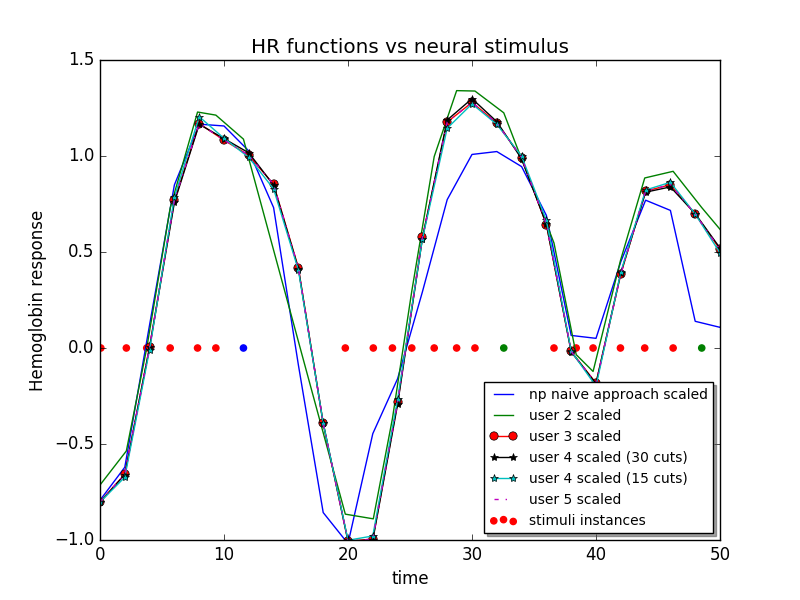
\includegraphics[width=.8\linewidth]{../images/convolution_vs_neural_stimulus}
		% needs to be from the event_related_HRF_script2.py 
		\caption{\scriptsize{Different convolution functions vs. the Neural stimulus}}
		\label{fig:convolution_a}

	\end{minipage}
\quad
	\begin{minipage}[b]{0.45\linewidth}
		\centering
		\begin{tabular}{|l | c|}
		\hline
		name in graph       & Speed per loop \\
		\hline
		np naive approach & 14.4 $\mu$s  \\
		user 2     		    & 972 ms  \\
		user 3     		    & 1.15 s    \\
		user 4 (15 cuts)      & 98.3 ms \\
		user 4 (30 cuts)      & 185 ms  \\
		user 5     	 	    & 110 ms   \\
		\hline
		\end{tabular}
		\vspace{5mm}
		\label{tab:convolution_a}
		\captionof{table}{\scriptsize{Speed to create HRF predictions for 
		Subject 001, all conditions}}
	\end{minipage}
\end{figure}

\par \noindent The first method in the table, ``np naive approach'', blindly 
plugs our data into the \texttt{np.convolve} function. It is provided to 
showcase potential speed. The failure of the "np naive approach" was the 
motivating factor behind the rest of the hemodynamic response convolution 
analysis, due to a lack of equidistant spacing of stimulus and scans. The 
``user 2'' and ``user 3'' functions runs fall under subcategory 
\textbf{(1)}. ``user 2'' was the first approach to
match the theory, but it matches the stimulation times and not the scan times.
``user 3'' is the most theoretically sound model (and is our standard for 
accuracy). The ``user 5'' falls under subcategory \textbf{(2)}, ``User 5''  is
our matrix version of the theory, and has the same accuracy as ``user 3''. The 
``user 4'' models falls under subcategory \textbf{(3)}, the methods that use the
grid cut usage of \texttt{np.convolve} with notations for the number of slices 
between each scan. We concluded that "user 4 (15 cuts)" was the best approach 
since it gives us speed and very close accuracy to the golden standard - ``user 
3".

\subsubsection{Time Correction}

\par \indent The fMRI machine scans each voxel at a slightly different time. 
In our case, the lowest horizontal slice was scanned first, with the later 
scans obtained in order progressively toward the top of the brain. The signs 
of this linear change in time of scan was observed when running simple 
regression on the data and found that the hemodyamic response $\hat{\beta}$ 
values from all conditions grouped together. We corrected for the time 
differences by shifting the times of stimuli ``backwards'' for voxels scanned 
later to directly correct for the delay of the scan (assuming that each layer 
of the scan took 2/34 of a second).

\subsubsection{Multiple Conditions}

\par \indent Originally, we used multiple regression to acount for the 
three different types of stimulus (pump, explode, cash-out) and examine if the 
separation of these stimuli can better describe the response. We did this by 
creating separate predicted hemodynamic reponses for each condition to allow 
for different amplitudes for each type of condition. As will be noted in 
Section \ref{model_selection} portion later, we did not observe a large 
difference in the results values we obtained, so we did not continue with 
this exploration. In Figure \ref{fig:all_cond_time}, we can see the different 
conditions separated the responses for each condition.
 

\begin{figure}[ht]
\centering
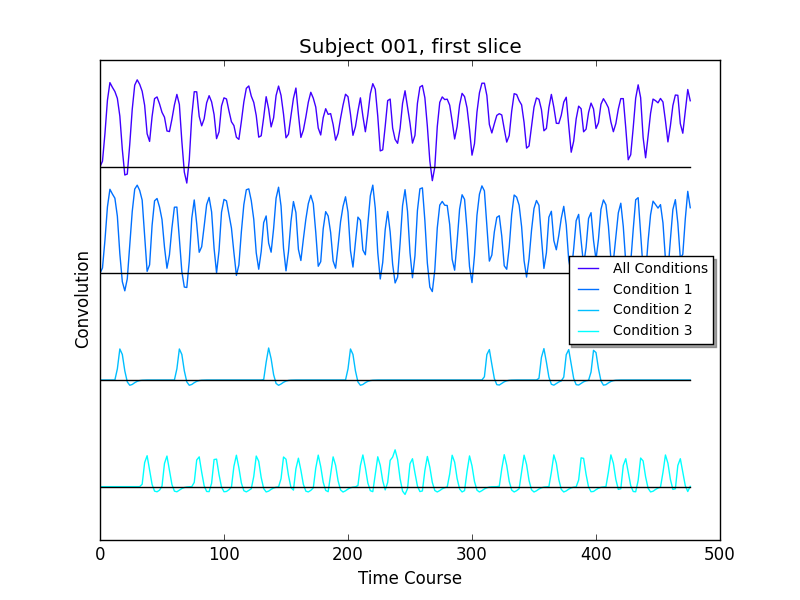
\includegraphics[scale=.5]{../images/all_cond_time}  
\caption{Plotting all predicted HR for conditions.}
\label{fig:all_cond_time}
\end{figure}

A more detailed discussion about our approach and the theory behind convolution 
of the hemodynamic response with the neurological response can be found 
in Appendix \ref{app_convolution}.


		
	\subsection{Linear Regression}
	
		% tex file for regression

	\subsection{Normality Assumptions}
	
		% tex file for normality
\par \indent The validity of our hypothesis tests for the estimated 
$\hat{\beta}$ values from the chosen linear regression model are largely 
dependent on whether we can reasonably assume that the errors in our model 
are independent and identically distributed from some normal distribution 
with mean zero and constant variance. We focus here on checking the normality 
assumption. It is generally wise to use visualizations, such as residual vs. 
fitted values plots and quantile-quantile plots to inspect residuals for 
patterns and abnormalities. However, considering the sheer quantity of data 
we are working with --- each of the 24 subjects has 64 $\times$ 64 $\times$ 34 
voxels that can each in turn be fitted to a model --- visual inspection is 
not practical. 

For this reason, we used the Shapiro-Wilk test for normality, 
which tests the null hypothesis that the data in question is normally 
distributed. A Shapiro-Wilk test was performed for each set of residuals 
corresponding to a single voxel's time course. That is, each test used around 
200 observations, or the number of time points for that particular subject. 
200 observations is not an especially large sample size, and for this reason, 
we express some concern because normality tests have low power for small 
sample sizes. Shapiro-Wilk may incorrectly fail to reject the null hypothesis 
due to this bias \cite{ghasemi2012normality}. 

The average proportion of Shaprio-Wilk test ``p-values'' above 0.05 was 0.742 
for the unmasked residuals across both subjects and voxels and noticeably 
lower at 0.630 for the masked residuals. However, since using the masked data 
is more theoretically justifiable (the unmasked data contains many voxels 
outside of the brain), we use the masked data for our analysis despite the 
lower proportion of voxels whose residuals meet our normality check. Note that 
these proportions suggest that only about two-thirds of the masked voxels have 
residuals that are approximately normal, and that the others deviate 
significantly from the normal distribution (especially when considering our 
concerns about the power of Shaprio-Wilk tests for small sample sizes). So when 
discussing our models and especially when looking at the conclusions made by 
our hypothesis tests, one should exercise caution about the validity of those 
conjectures. 

Figures \ref{fig:sw} and \ref{fig:sw_masked} compare the spatial distribution 
of the Shapiro-Wilk ``p-values'' for Subject 10's masked and unmasked data. 
The unmasked figure is very difficult to interpret, but the masked figure does 
suggest that while the spatial distribution of voxels with approximately 
normal residuals is reasonably uniform in many regions, there are a few areas 
that consistently have very low ``p-values'' at around or below the 0.05 
threshold. Examples of these regions for Subject 10 include a small area 
between the front and center of the brain and a few spots near the sides. 
However, these observations are not consistent across all subjects, so much 
of it may simply be due to noise. 

\begin{figure}[ht]
\centering
\begin{minipage}[b]{0.45\linewidth}
	\centering
	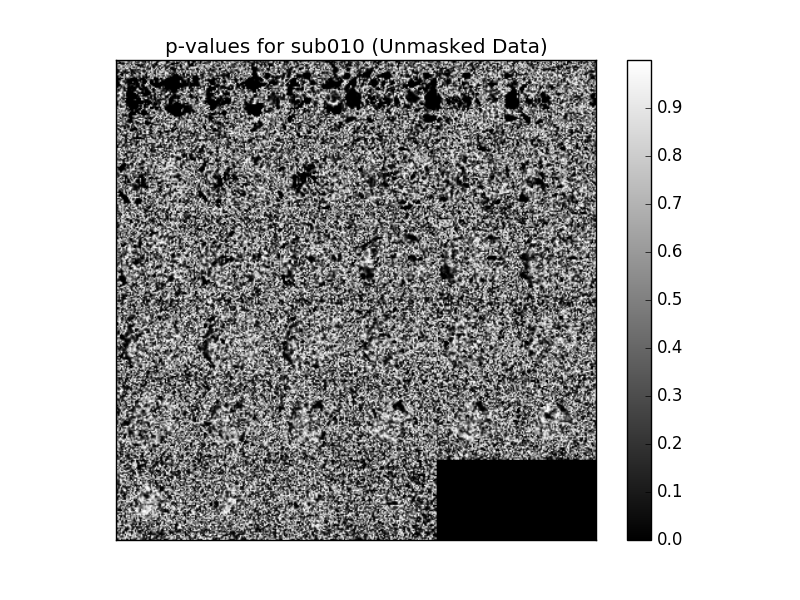
\includegraphics[width=.8\linewidth]{../images/sub010sw.png} 
	\caption{Subject 10's brain slices, with voxels colored by the magnitude of the
``p-value'' in the corresponding Shapiro-Wilk test for normality.Using unmasked residuals.}
\label{fig:sw}
\end{minipage}	
\quad
\begin{minipage}[b]{0.45\linewidth}
	\centering
		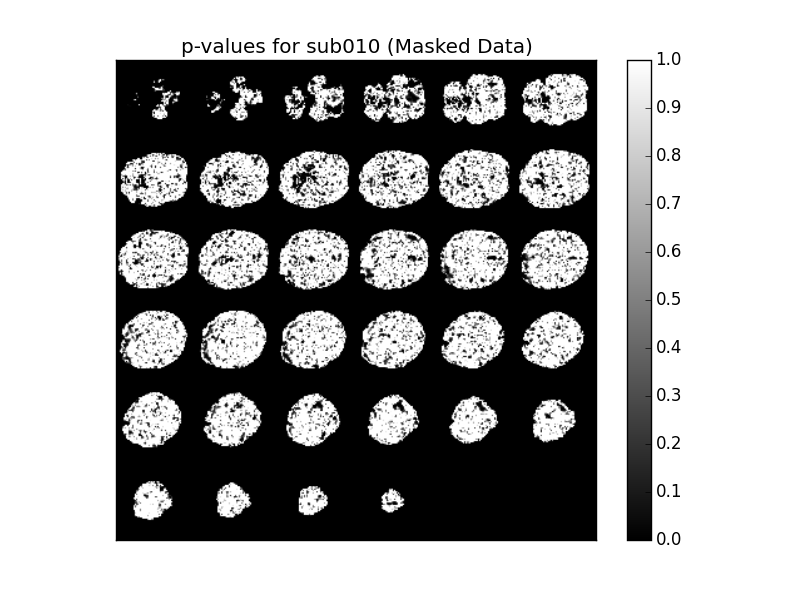
\includegraphics[width=.8\linewidth]{../images/sub010swmasked.png} 
	\caption{Subject 10's brain slices, with voxels colored by the magnitude of the
``p-value'' in the corresponding Shapiro-Wilk test for normality. Using masked residuals.}
\label{fig:sw_masked}
\end{minipage}
\end{figure}

		
	\subsection{Hypothesis Testing} \label{hypothesis_testing}
	
		% tex file for hypothesis 
\par \indent Our simple linear regression model was created to better 
understand the relationship between the voxels in a given subject's brain and 
the convolved time course. In order to measure the strength of the association 
between these two measurements, we ran a hypothesis test on the coefficients of 
the simple linear regression model for each subject. 

\par There is an individual linear model associated with each voxel in a
subject’s image (and a total of $64 \times 64 \times 34$ voxels per subject).
Thus we ran a t-test on each voxel's $\beta$ coefficient that is associated
with the HRF response. The null hypothesis for each test was that $ \beta = 0$,
with the alternative hypothesis that $\beta \neq 0$. Once we had obtained each
t-statistic, we compared this value across voxels in two ways. First, we simply
compared this t-values with voxels within a subject. In this case, we took into
account the sign of the t-statistic in our analysis. Second, we converted this
t-statistic to a "p-value", in which case the sign of the t-value will become
irrelevant and we compared across voxels without taking into account this sign.
Later, we also run a multiple comparison test using a Benjamini\–Hochberg in
order to find the voxels that are most significant.


\par Having implemented a method to compare the voxels within a single subject, 
we next examined our results for the same voxels across subjects. Our initial 
approach was to aggregate the t-statistic data between all subjects for each 
voxel. This allowed us to decrease the variability of the fit on each voxel and 
detect a more clear signal. 

\par In order to do this, we ran the hypothesis test as stated above on all 24 
subjects of the study. Then for each voxel, we took the average of the t-
statistics across the subjects. An issue with our data was the presence of 
empty space detected by the scanner that is not directly part of the brain. To 
account for this, we took the masked data of the brain and ``cut out'' the parts 
of the images that were not relevant to our analysis. Ultimately, we were left with 
a single 3-d image with each voxel representing the average t-statistics across 
all subjects in the study. This image will later be used in our clustering step in 
order to pinpoint the regions of the brain that have the strongest relationship 
with the convolved time course. 


	\subsection{Clustering}
	
		% tex file for clustering 
\par Now that we have the across subject average t-values for every voxel in
the brain, we are left with a 3d array of t-values that contain both negative
and positive values. Instead of manually observing patterns in these images, we
instead impelmented a clustering algorithm to split the entire 3d images into
clusters based on the voxels' relative location to each other as well as the
t-value.

\par In order to find a proper clustering algorithm, we decided to treat this
problem like a grayscale image segmentation problem and implemented a
agglomerative hierarchical cluster using Ward's method. Agglomerative means
that the clusters are built bottom up which each observation starting as its
own cluster and pairs being moved up the hierarchy. Ward's method creates
clusters based on a minimum variance criterion that miniizes the total
within-cluster variances. An example of this implimentation for a 2d image is
seen here: 
\url{http://scikit-learn.org/stable/auto_examples/cluster/plot_lena_ward_segment
 ation.html}.

In our implimentation, we defined a structure to our data using a connectivity
graph in order to ensure that each cluster is spatially constrained. Also,
since our scenario uses a 3d image, the connectivity graph will also have to
take into account this extra dimension.

\par Ultimately, the goal of this clustering is to have a better understanding
of which parts of the brain are related to the signal based on its t-values.
Once we obtain our clusters, we will both measure the within-cluster mean of
t-values as well measure the centroids of the clusters. By doing this, we hope
to see the parts of the brain that have the strongest relationship with the
signal and compare them to the results of the origin alresearch paper.




		
\section{Results} \label{results}
		
	% tex file for results

% from regression_results

\noindent \textbf{Pre-Processing}

Smoothing performed well in reducing outliers and extreme values in the time-series per voxel. We used a value of $\sigma=1$ for the Gaussian smoothing.  We performed HRF convolution and time correction as well with success.
\vspace{5mm}

\noindent \textbf{Model Selection}

For our linear regression model, we ended up choosing the deisgn matrix model with a single HRF feature with all conditions, a linear drift feature, and three pairs of Fourier features. The dimension of our final feature matrix is time $\times$ 9. 
\vspace{5mm}

\noindent \textbf{Normality Test}

Based on the Shapiro-Wilk test for normality on the residuals with a p-value threshold of 0.05, we found that the normality assumptions of the linear models were violated roughly 35\% of the time. This suggests that we should be cautious of the validity of hypothesis testing and possibly explore alternatives for analyzing the coefficients.
\vspace{5mm}

\noindent \textbf{Clustering}

Our end goal was to identify regions of the brain that are associated with the neurological stimulus by way of the hemodynamic response. In pursuing this goal, we utilized the $\hat{\beta}$ and t-statistics corresponding to the HRF coefficient of the chosen linear model design matrix. Based on the fact that the normality assumptions did not hold for a large proportion of the voxels, we utilized analyses that both relied and did not rely on the normality assumption.

We used two perspectives to cluster, one based of multiple correction and another based on hierarchical clustering using Ward's method. Hierarchical clustering was computationally costly against the large number of voxels and was not feasible. We used 3 different approaches to multiple comparison correction. 
\vspace{5mm}

\noindent \textbf{Multiple Comparison}

The most canonical appraoch we used was Benjamini Hochberg (BH), which utilized p-statistics. This type of analysis assumes normality of the $\hat{\beta}$ values, which we saw where not always the case. BH also required unique threshold values for each person, which was a large draw-back. We additionally utilized a quantile-based clustering of the t-stat values and $\hat{\beta}$ values. These provided more interpretable clusters across subjects and produced similar results indicating consistency.
\vspace{5mm}

\noindent \textbf{Identifying Active Regions}

We considered the results from each of the approaches for clustering with multiple comparison corrections. As alluded to previously, the BH approach was less interpretable and required per-subject tuning of parameters to obtain logical results. So, it was generally a less favorable approach than the t-statistic and $\hat{\beta}$ quantile-based clustering. 

Sub 1, Kent's actual, 
[Some plots here for at least 2 subjects with consistent results and at least 1 subject with weird results. Ideally should also compare methods to demonstrate the similarities between t and beta and the weirdness of BH.]

A region consistently identified with high HRF activity across subjects for the t-statistic and $\hat{\beta}$ approaches was the front area of the brain. Other areas with potentially high activity include a small region toward the center and back and some areas on the left edge. 
\vspace{5mm}


\begin{figure}[ht]
\centering
\begin{minipage}[b]{0.45\linewidth}
	\centering
	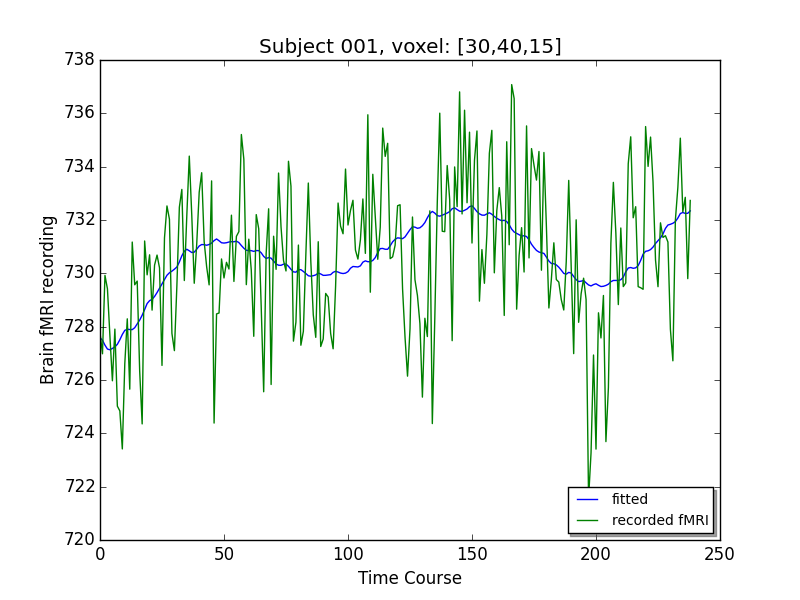
\includegraphics[width=.8\linewidth]{../images/Fitted_v_Actual.png} 
	\caption{Fitted/Predicted vs Actual fMRI BOLD contrast}
	\label{fig:fit_vs_act}
\end{minipage}	
\quad
\begin{minipage}[b]{0.45\linewidth}
	\centering
		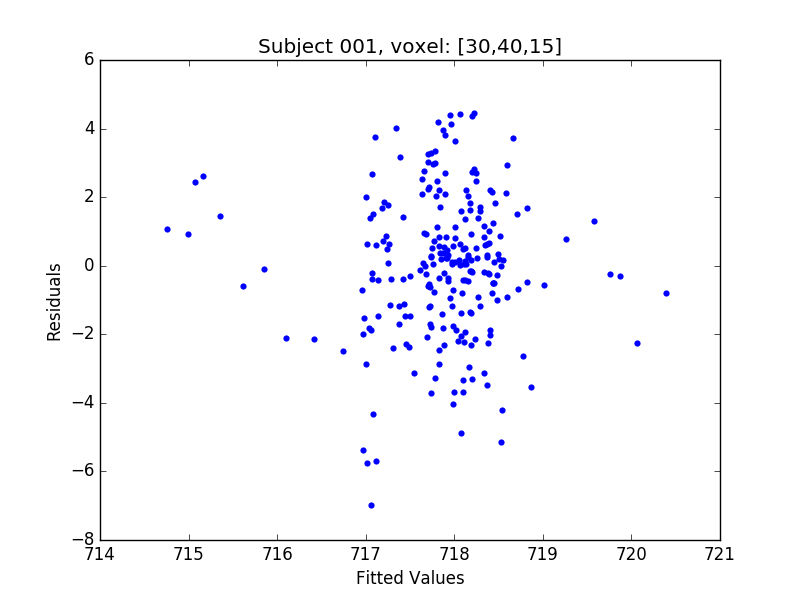
\includegraphics[width=.8\linewidth]{../images/Fitted_v_Residuals.png} 
	\caption{Fitted fMRI BOLD contrast vs Residual from Linear Regression}
	\label{fig:fit_vs_res}
\end{minipage}
\end{figure}





  
\begin{figure}[ht]
\centering
\begin{minipage}[b]{0.45\linewidth}
	\centering
	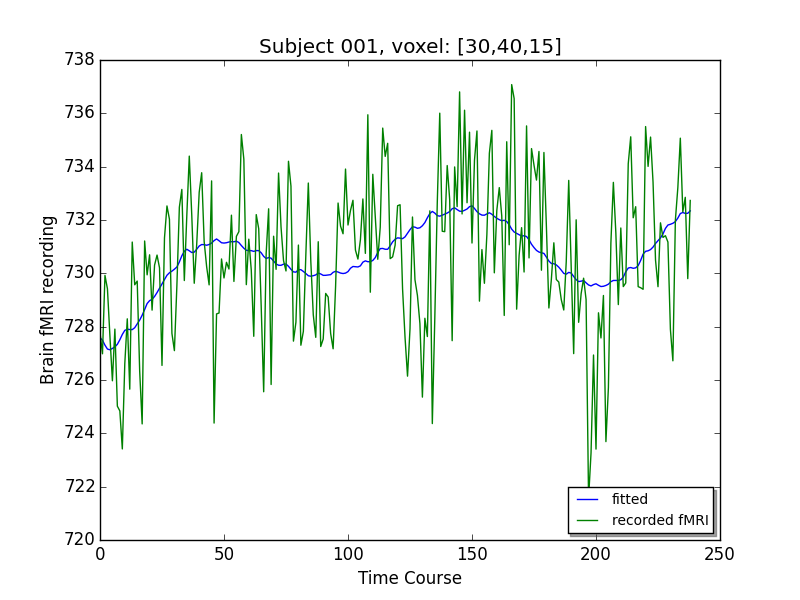
\includegraphics[width=.8\linewidth]{../images/Fitted_v_Actual.png} 
	\caption{Fitted/Predicted vs Actual fMRI BOLD contrast}
	\label{fig:fit_vs_act}
\end{minipage}	
\quad
\begin{minipage}[b]{0.45\linewidth}
	\centering
		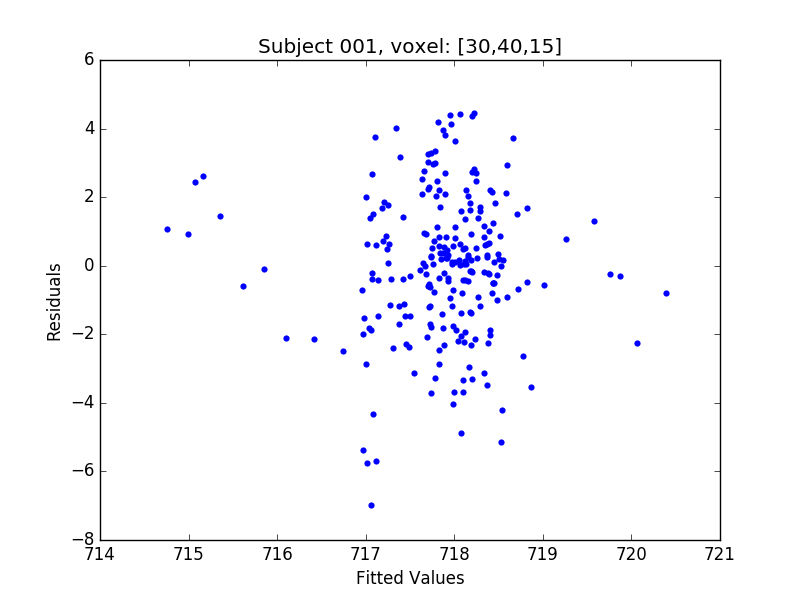
\includegraphics[width=.8\linewidth]{../images/Fitted_v_Residuals.png} 
	\caption{Fitted fMRI BOLD contrast vs Residual from Linear Regression}
	\label{fig:fit_vs_res}
\end{minipage}
\end{figure}




%\begin{figure}[ht]
%\centering
%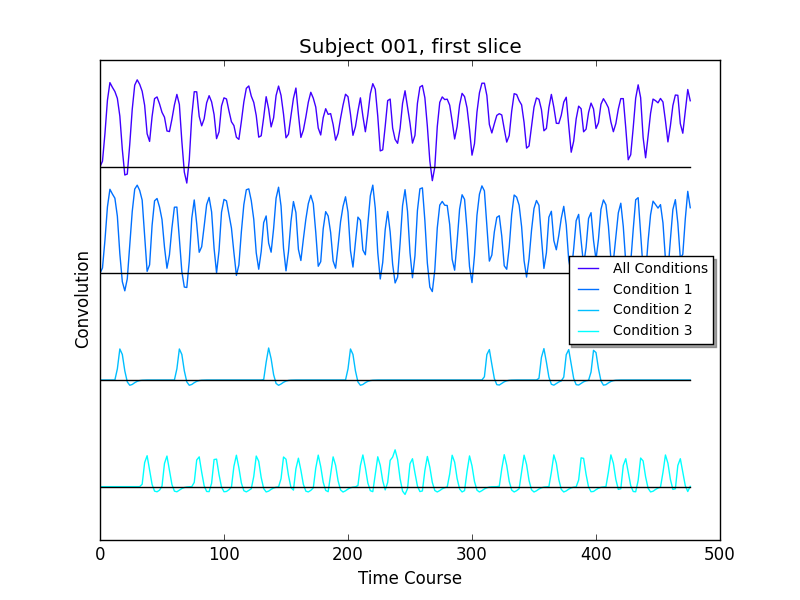
\includegraphics[scale=.5]{../images/all_cond_time}  
%\caption{Plotting all predicted HR for conditions.}
%\label{fig:all_cond_time}
%\end{figure}

*****As we also obtained $\hat{\beta}$ values (coefficients) from the linear 
regression models, we looked at the 3-dimensional reports of the 
$\hat{\beta}$ values, a less rigorous analysis than hypothesis testing with 
t-statistics [Figure reference]. $\sim$Remove or update****



The numerous other multiple regression models discussed in 
\textit{Linear Regression} should be analyzed similarly in the future. 



% from hypothesis_results
% tex file for hypothesis testing results 
\par \indent The results of our simple linear regression t-statistic 
comparisons across subjects are shown in [Figure \ref{fig:ht}]. We can see 
each slice of the brain from top to bottom in each section of the image. The 
blue areas shows parts of the brain that had a negative t-statistic while the 
red parts of the image shows parts of the brain that had a positive t-
statistic.

\begin{figure}[ht] \centering
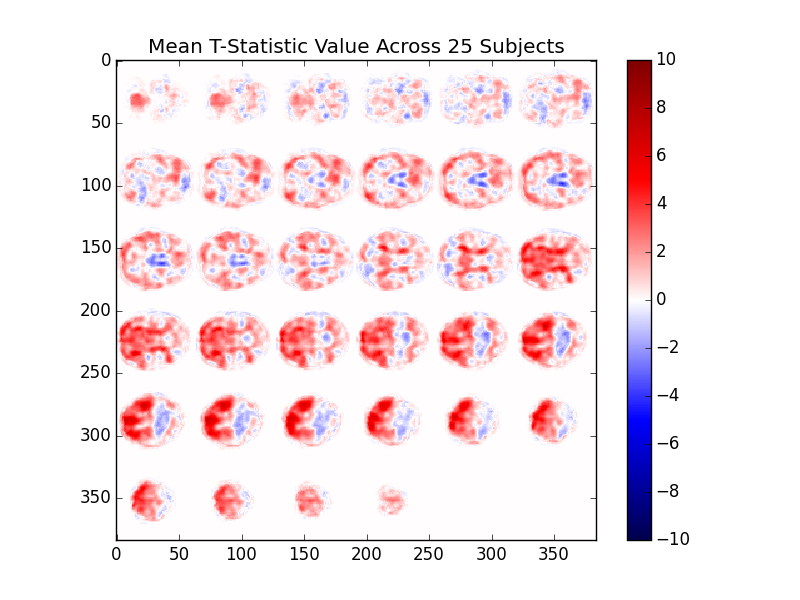
\includegraphics[scale=0.5]{../images/hypothesis_testing} \caption{Across-subject 
mean of t-Statistic per voxel.} \label{fig:ht} \end{figure}

\par The parts of the image that were cut out by the mask are white so we can 
more clearly see the contrast in our results. Based on a cursory look at this 
image, we can see a pattern of dark red (high positive t-statistics) in the lower 
left parts of the brain, and area of dark blue (high negative t-statistics) in 
the center and lower middle parts parts of the brain.




\section{Discussion} \label{discussion}
	
	\subsection{Discussion of Results}
		
		% tex file for discussion
\par \indent While very much still a work in progress, our analysis thus far 
includes methods for both data processing and modeling voxel time courses. 
Prior to doing any serious analysis, we had to smooth the data spatially for 
each subject. We also generated a reasonable convolved time course with time 
shift corrections, based on event-related neurological stimuli with 
non-constant intervals. 

\par A basic but nevertheless important model to consider is linear regression. 
We implemented both simple and multiple regression models at the individual 
subject level. In addition to the convolved time course, our multiple linear 
regression models attempt to account for more of the noise in our data by 
including terms for event conditions, linear drift, and discrete cosine 
transforms. We then checked the assumptions for the fitted models and performed 
hypothesis testing on the resulting coefficients for each voxel. Though the 
linear regression models were designed to handle each voxel for each subject's 
data individually, we aggregated the data across the 24 subjects by taking the 
means of the t-statistics corresponding to each voxel. However, one major concern 
for hypothesis testing is the issue of multiple comparisons, which we attempted to 
address using the Benjamini-Hochberg procedure. Finally, we used k-means 
clustering to further identify areas of the brain with high neurological activity 
during the events of the BART study. 




		
	\subsection{Discussion of Future Work}
	
		% tex file for future discussion
\par \indent The implementation of permutation tests, which have few 
assumptions and are easy to interpret (but computationally intensive), 
would have been useful for testing the significance of the estimated 
coefficients from linear modeling. This can serve as an alternative to 
t-tests, which make several assumptsion about the data structure. 
Somewhat relatedly, additional tests and checks for model assumptions would 
also be valuable for assessing the appropriateness of our existing hypothesis 
testing. 

\par One major issue that we were unable to fully address is how to 
appropriately aggregate the results from individual subjects to make more 
general conclusions about activation regions, as opposed to the 
activation region of a particular subject. Much of this is due to the 
considerable variety in brain positioning and shape observed between different 
subjects; there is really no such thing as an ``average'' subject. One 
approach that we tried was to simply average across subjects the binary 
t-statistic masks from the quantile-based clustering (Figure \ref{fig:avgt}). 
The result was a single ``average'' brain, but since there is considerable 
variance in brain size, shape, and so on, the justification for this method 
was not theoretically sound. Nevertheless, having that single average brain 
makes interpretation easier. For our situation, this method was able to tease 
out the high activity in the back of the brain, but not elsewhere. 

\begin{figure}[ht]
\centering
	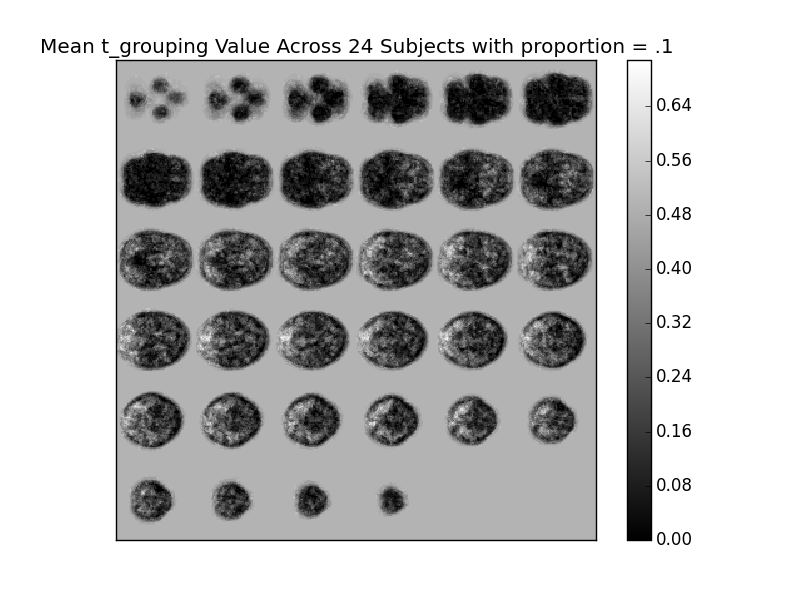
\includegraphics[width=.8\linewidth]{../images/tgroup_mean_final.png} 
	\caption{Slices from averaging the binary t-statistic masks across 
subjects. Colors indicate the proportion of subjects that identified a voxel 
as significant.}
	\label{fig:avgt}
\end{figure}

\par Additional future work could also be concerned with reproducing our 
approach for identifying actived regions on the pre-cleaned version of the 
study's data provided by the organizers of the OpenfMRI project. Those results 
could then be compared with the results from using our own pre-processing 
techniques. Since fMRI data is notoriously noisy, the different decisions made 
when cleaning the data to seperate the signal from the noise can greatly alter 
the results. So while ideally, both our pre-processed data and the 
alternatively pre-processed data would identify the same active regions, we 
acknowledge that there is a reasonably high chance that this would not be the 
case. 

\par Relating back to the issue of aggregating subjects, one great advantage 
to using the cleaned data from Ross Poldrack and the OpenfMRI project is that 
the subjects were registrated to a standard MNI anatomical template. Averaging 
clustering results across subjects would make more sense here, since the 
standard template should account for many of the differences in brain shape 
and positioning in the fMRI scanner. Near the end of our project we attempted
to incorporate the new data, but with 8 $\times$ as much data per subject and 
the nonlinear order of growths caused problems in the short term.


\pagebreak

		%%%%%%
% Final plots from results



\begin{figure}[H]
\centering
\begin{minipage}[b]{.66\linewidth}
	\centering
	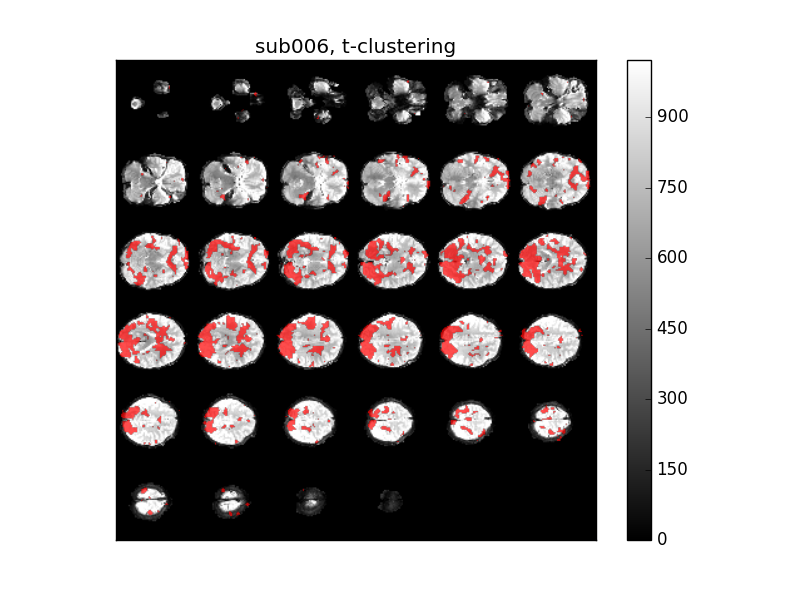
\includegraphics[width=.8\linewidth]{../images/sub006_t_overlay.png} 
	\caption{Quantile-based clustering for Subject 6's t-statistics. 
	(Red areas denote significant regions)}
	\label{fig:clustert}
\end{minipage}	

\begin{minipage}[b]{.66\linewidth}
	\centering
		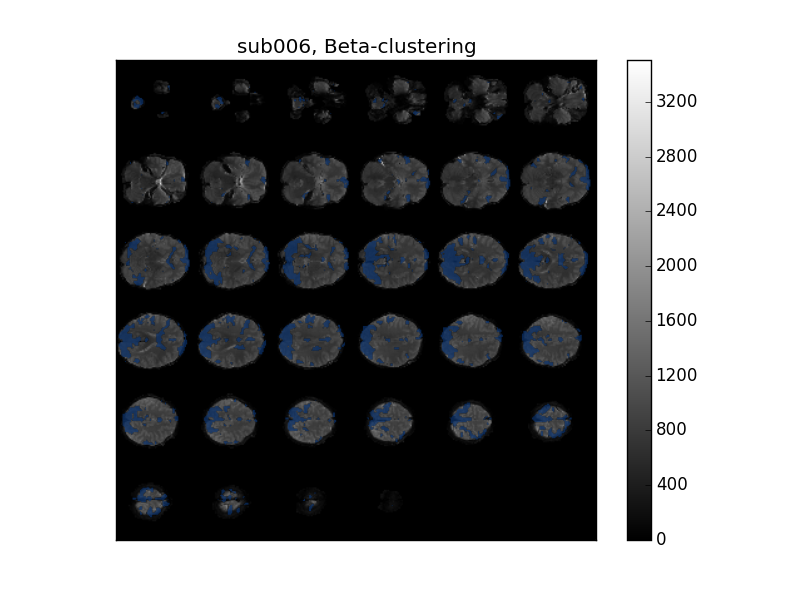
\includegraphics[width=.8\linewidth]{../images/sub006_beta_overlay.png} 
	\caption{Quantile-based clustering for Subject 6's $\hat{\beta}$ coefficients. 
	(Red areas denote significant regions)}
	\label{fig:clusterbeta}
\end{minipage}

\begin{minipage}[b]{.66\linewidth}
	\centering
		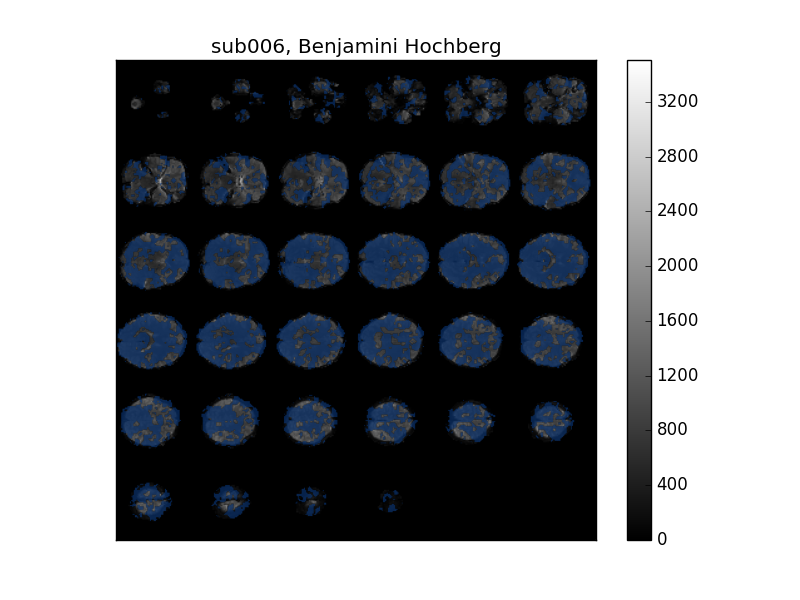
\includegraphics[width=.8\linewidth]{../images/sub006_bh_overlay.png} 
	\caption{Benjamini-Hochberg clustering for Subject 6. 
	(Red areas denote significant regions)}
	\label{fig:clusterBH}
\end{minipage}
\end{figure}


\begin{figure}[H]
\centering
\begin{minipage}[b]{.66\linewidth}
	\centering
	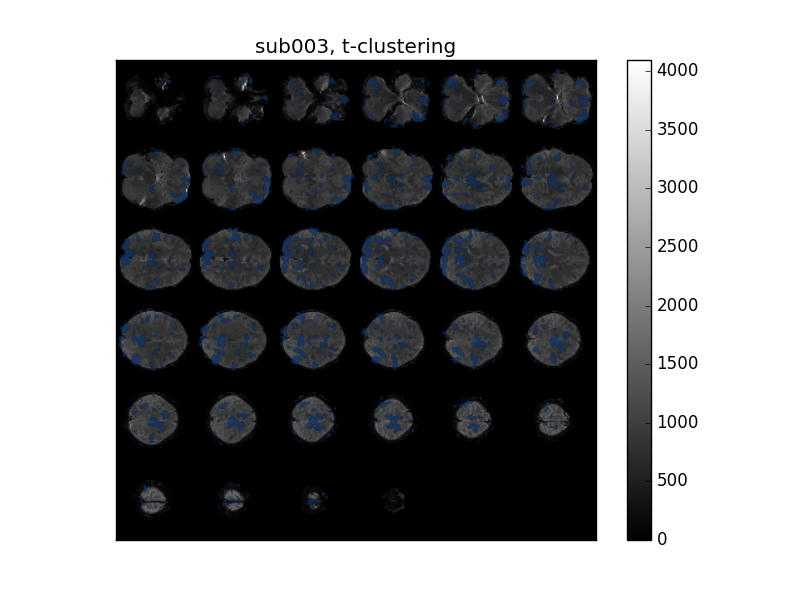
\includegraphics[width=.8\linewidth]{../images/sub003_t_overlay.png} 
	\caption{Quantile-based clustering for Subject 3's t-statistics. 
	(Red areas denote significant regions)}
	\label{fig:clustersub3}
\end{minipage}	

\begin{minipage}[b]{.66\linewidth}
	\centering
		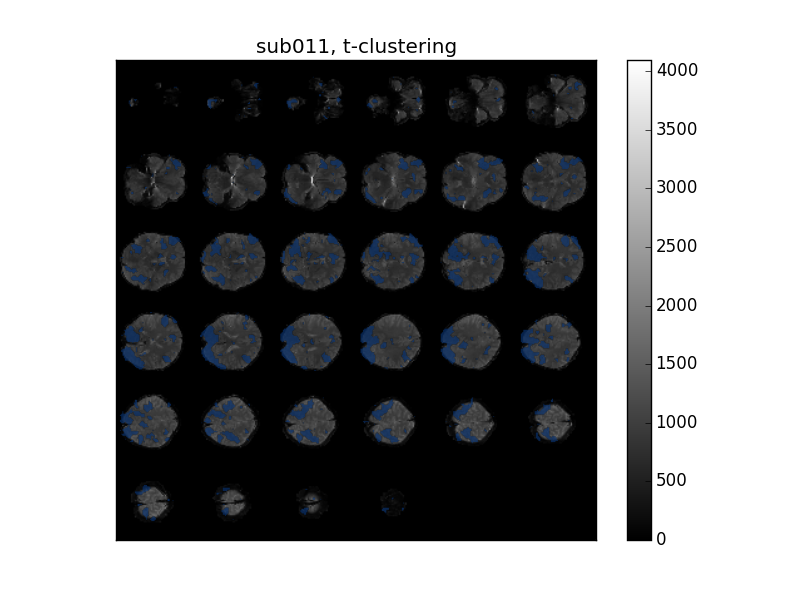
\includegraphics[width=.8\linewidth]{../images/sub011_t_overlay.png} 
	\caption{Quantile-based clustering for Subject 11's t-statistics. 
	(Red areas denote significant regions)}
	\label{fig:clustersub11}
\end{minipage}

\begin{minipage}[b]{0.66\linewidth}
	\centering
		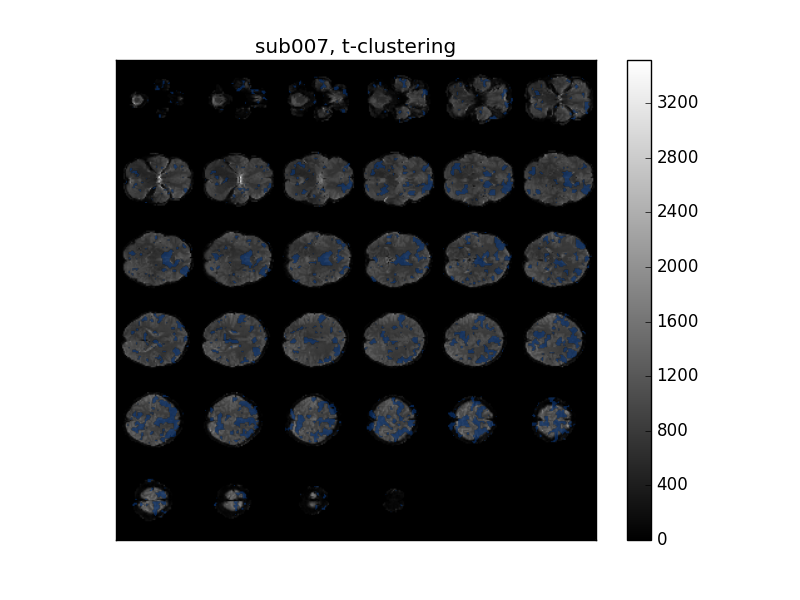
\includegraphics[width=.8\linewidth]{../images/sub007_t_overlay.png} 
	\caption{Quantile-based clustering for Subject 7's t-statistics. 
	(Red areas denote significant regions)}
	\label{fig:clustersub7}
\end{minipage}
\end{figure}






\pagebreak

\begin{center}
\Huge{Appendix} \appendix
\end{center}


\section{Outlier Removal} \label{app_outliers}

\documentclass[11pt]{article}

\usepackage[margin=0.75in]{geometry}
\usepackage{indentfirst}
\usepackage{graphicx}
\usepackage{hyperref}
\bibliographystyle{siam}

\title{Appendix: Outlier Removal}
\author{
  Liang, Jane\\
  \texttt{janewliang}
}

\begin{document}
\maketitle

We considered following the procedure implemented as part of Homework 2 to 
detect and remove outlier 3-d volumes from the 4-d image scans of each subject. 
The process involves finding the root mean squares (RMS) of each 3-d volume 
across time and then getting the difference values. When a given volume is very 
different from the preceding volume, this may indicate a potential outlier or 
the sign of an artifact. We used thresholds based on 1.5 $\times$ IQR added to 
the 75th percentile and subtracted from the 25th percentile to create the 
cutoffs for the RMS difference outliers. We then extended the RMS difference 
outliers by labeling the volumes either side of the outlier RMS difference as 
being outliers. 

Each subject was considered independently, as considerable variation in 
measurement is expected between different subjects. However, we found that 
reductions in mean residual sum of squares from running simple linear regression 
before and after removing the extended RMS difference outliers were minimal. 
Visually speaking, we also did not observe the presence of egregiously different 
points. So, we opted to refrain from removing outliers, at least through the 
extended RMS difference method. 

\bibliography{project}

\end{document}


\section{Smoothing} \label{app_smoothing}

\documentclass[11pt]{article}

\usepackage[margin=0.75in]{geometry}
\usepackage{indentfirst}
\usepackage{graphicx}
\bibliographystyle{siam}

\title{Appendix: Smoothing}
\author{
  Lee, Rachel\\
  \texttt{reychil}
}

\begin{document}
\maketitle

\par \indent We used a Gaussian filter to smooth away noise in the brain 
images. At first, we played around with implementing a function similar 
to a mean filter, where each voxel would be the average of a certain radius 
of its neighbors. Ultimately, we decided to use a kernel with a Gaussian 
(bell-like) shape. 

\par The property that makes the Gaussian filter a stronger and more 
reliable candidate for smoothing the voxel data is that it outputs a weighted 
average of the voxel and its neighbors. The more heavily weighted values are 
at the center of each of the neighborhood of voxels we examine. On the other 
hand, a regular mean filter would use a uniformly weighted average, which 
means that there is the risk of oversmoothing, along with additional 
complications of handling the voxels along the edges of the brain image data. 
Furthermore, a Gaussian filter is ideal for use in noisy voxel data because of 
its steady frequency response. By choosing an appropriate filter, we have can 
gain more control of the range of spatial frequencies left after smoothing 
the data. Additionally, Gaussian filters are non-negative for all voxel data. 
Thus, the output of smoothing the voxel data with a Gaussian filter will still 
be a valid image. 

\par In conclusion, we decided to go with the module for a Gaussian filter for 
several reasons, the main one being that Gaussian filters can remove noise and 
yet preserve the high frequency edges in the brain image data. Rather than use 
a self-implemented mean filter function that would cause issues with high-
frequency edge cases as well as conglomerating data into thoughtless averages, 
a Gaussian filter handles these situations better because the smooth, bell-
shaped curve of the convolution does not have a sharp cutoff at edges. The 
Gaussian filter also distributes weighted averages across the voxels such that 
the smoothing keeps high-frequency data points into consideration for the end 
product.

\bibliography{project}

\end{document}


\section{Convolution Analysis} \label{app_convolution}

% Convolution appendix. 

\subsection{Introduction}

fMRI data presents a distinct challenge for relating neural stimuli 
to BOLD (blood-oxygen-level dependent) response. fMRI scans record changes 
in oxygenation levels of hemoglobin in the brain. However, there is a delay 
between the neural stimulus and the change in blood oxygen levels in a given 
area. In our case, the neural stimulation comes from a event-related 
experimental design. A commonly assumed hemodynamic response to a neurological 
stimulus is the double gamma function that can be seen in Figure 
\ref{fig:hrf}. The complete hemodynamic response function needs to be modeled 
in order to better relate stimulation and the BOLD response from the fMRI scan.
It should be noted that the BOLD response is highly noisy and we are really 
trying to capture the blood oxygenation level change to the stimulation.

\subsection{Mathematics}
\subsubsection{Convolution Theory and Mathematics}

To relate stimuli to BOLD response, we convolved the time courses of discrete 
stimuli with the assumed response to a single stimulus. At a basic 
level, convolution is a distinct combination of two functions (say $f$ and 
$g$). This combination is just the ``integral that expresses the amount of 
overlap of $f$ as it is shifted over another function $g$'' 
\cite{weissten2015convolution}. 
There are many examples of this, but the following is basic idea that we will 
expand off of later. 

Let us define the function $f$ as a sum of two gamma functions and $g$ as a 
``continuous'' specialized step function (we will examine why these functions 
are valuable later). Graphically, we can see their plots in Figure \ref{fig:f}
and \ref{fig:g}, and mathematically we will define them as in the following 
equations \ref{eq:gamma2} and \ref{eq:step}, respectively.

\begin{equation} \label{eq:gamma2}
f(t)=\frac{.6}{.17}\cdot  \big[G_1(6,t)-.35 \cdot G_1(12,t) \big]
\end{equation}

where $G_1(k,t) =\frac{1}{\Gamma(k)} t^{k-1} e^{-t}$ (the gamma pdf with 
$\theta =1$)

\begin{equation} \label{eq:step}
 g(t)=\Big \{ \begin{tabular}{l c}
 		0  & if  5.85 $\leq$ t $\leq$ 6.15\\
 		.6  & otherwise \\
 		\end{tabular} \end{equation}
 		
 		
\begin{figure}[ht]
\centering
\begin{minipage}[b]{0.45\linewidth}
	\centering
	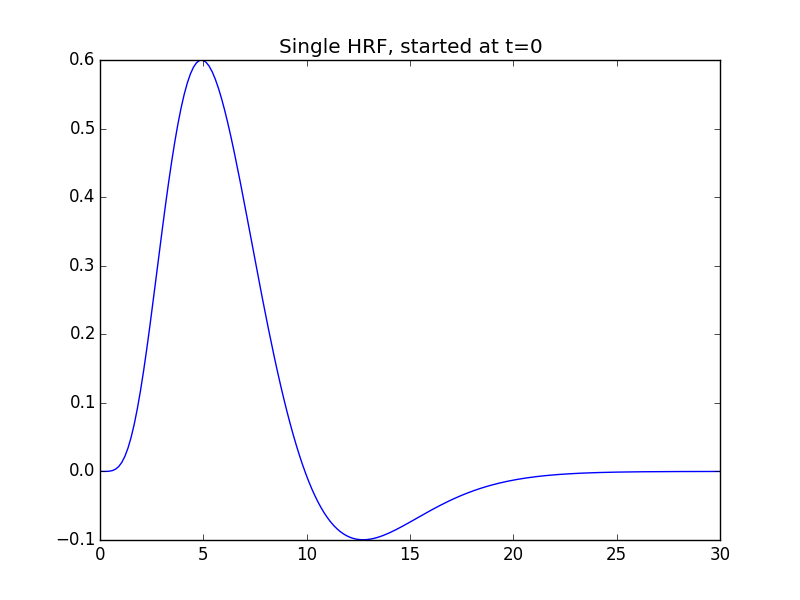
\includegraphics[width=.8\linewidth]{../images/hrf_pattern.png} 
	\caption{$f$ (``Stabilized Function'').}
	\label{fig:f}
\end{minipage}	
\quad
\begin{minipage}[b]{0.45\linewidth}
	\centering
		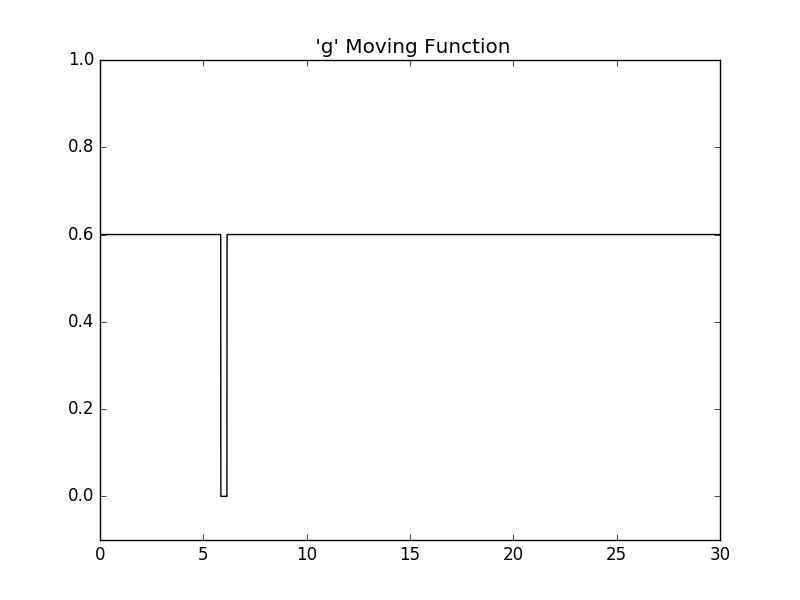
\includegraphics[width=.8\linewidth]{../images/play.png} 
	\caption{$g$ (``Moving function'').}
	\label{fig:g}
\end{minipage}
\end{figure}


As mentioned in the earlier definition, if we move $g$ across $f$ from 
left to right, we will see something similar to Figure \ref{fig:math} for 
discrete time intervals. If we plot these values (the integration of the 
differences), we will get a plot very similar to that of $f$ when $f$ is 
starting at a certain point. (The plot actually ``cheats'' when $f$ is 
negative, and we would have to alter definitions a little bit). If we had 
multiple peaks in our $g$ function (i.e. multiple distinct``zero'' places), we 
would expect to get multiple non-zero differences between the functions at 
each time capture. 

\begin{figure}[ht]
	\centering
	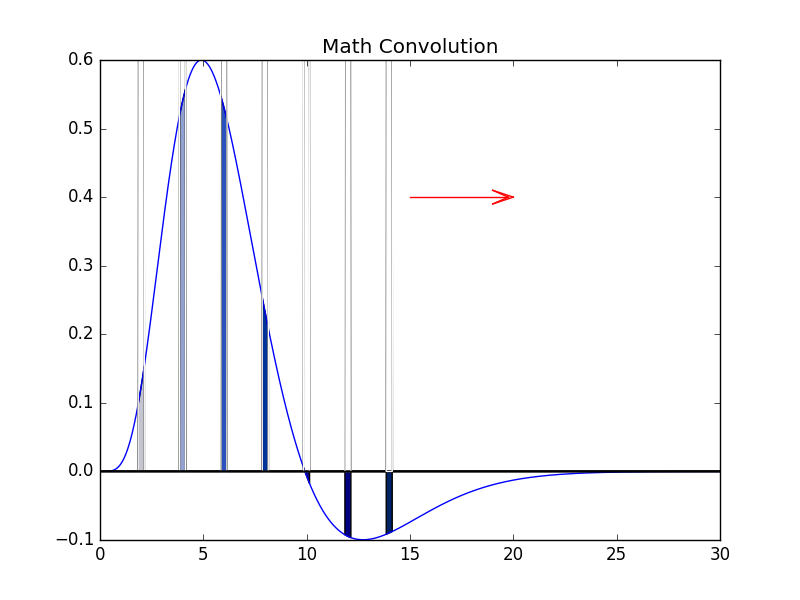
\includegraphics[width=.5\linewidth]{../images/math_convolved.png}
	\caption{Convolution of $f$ and $g$.}
	\label{fig:math}
\end{figure}


\subsubsection{Convolution Applied to Stimulus}

The ``continuous'' nature of the step function ``g'' does not extend well into 
the discrete time series that we have. However, one approach for fMRI analysis 
is to approach the convolution as something slightly different: mathematical 
sums. For example, in the previous section, we can treat $f$ as the same, and 
$g$ as $g'$ defined in equation \ref{eq:g_prime}.

\begin{equation}\label{eq:g_prime}
 g'(t)=\Big \{ \begin{tabular}{l c}
 		1  & if t=6\\
 		0  & otherwise \\
 		\end{tabular} \end{equation}

We could then find the value of the convolution of $g'$ and $f$ for discrete 
integers as in equation \ref{eq:math_discrete}.


\begin{equation}  \label{eq:math_discrete}
r(t)=  f(t-6)
\end{equation}



If we allow for multiple non-zero periods in $g'$, we can get a more general 
model in equation \ref{eq:math_discrete_extend}, where each $t_i$ is a value 
when $g'(t_i) \neq 0$: 

\begin{equation}  \label{eq:math_discrete_extend}
r(t)= \sum_{i=1}^n f(t-t_i)
\end{equation}

This equation gives a good glimpse into what the hemodynamic response would be 
after stimulus at time $t_i$ for $i \in {1,...,n}$. Moreover, one could extend 
the idea to include a ``strength'' value of the stimulus by changing the 
$g'(t_i)$ to values other than 1. If that was the case, we would change 
the response equation to Equation \ref{eq:math_discrete_final} to allow us to 
include all discrete $t$ into the equation where $g'(t_i)$ is now expected to 
be zero (so $n$ becomes much larger). 

\begin{equation}  \label{eq:math_discrete_final}
r(t)= \sum_{i=1}^n g'(t_i) f(t-t_i)
\end{equation}


With this new equation, we can consider function $f$ and $g'$ displayed 
graphically [Figure \ref{fig:hrf}, \ref{fig:on_off}, respectively] and 
their ``convolved'' output [Figure \ref{fig:convolve1}].




\begin{figure}[ht]
\centering
\begin{minipage}[b]{0.45\linewidth}
	\centering
	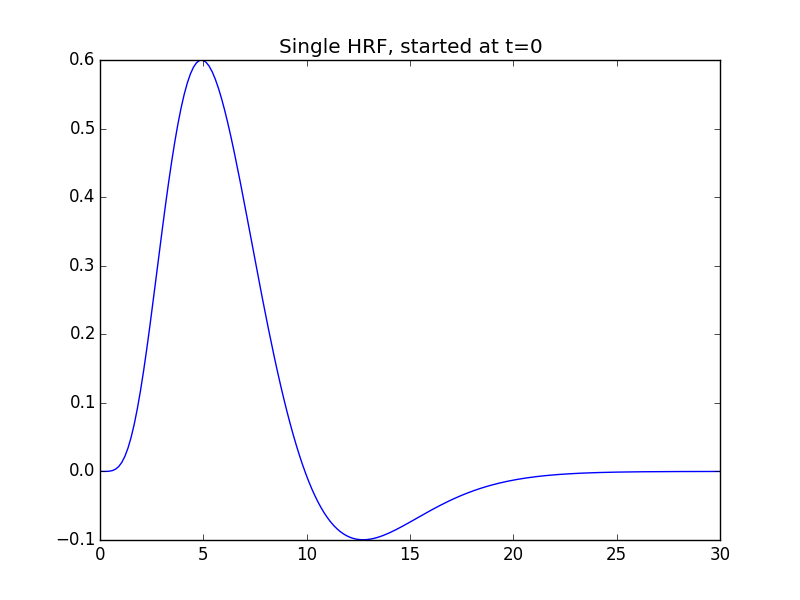
\includegraphics[width=.8\linewidth]{../images/hrf_pattern.png} 
	\caption{$f$ (``Stabilized Function'').}
	\label{fig:hrf}
\end{minipage}	
\quad
\begin{minipage}[b]{0.45\linewidth}
	\centering
	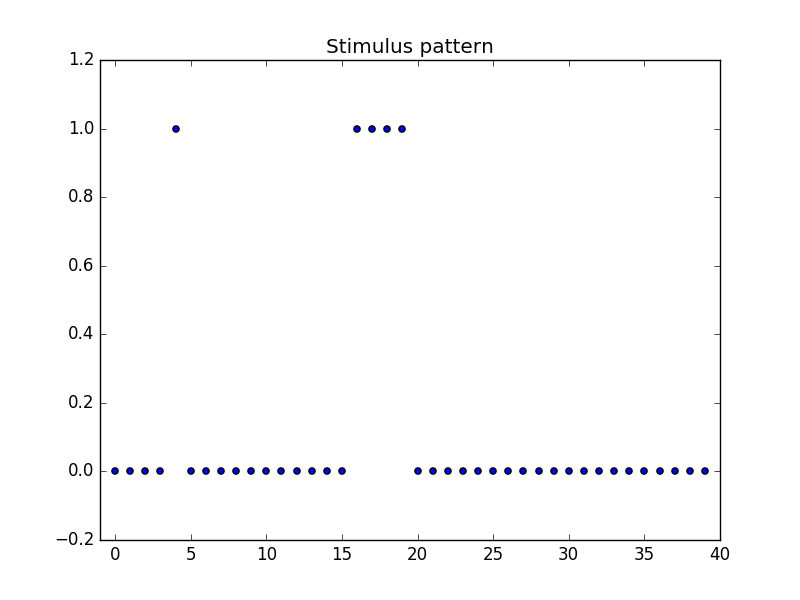
\includegraphics[width=.8\linewidth]{../images/on_off_pattern.png} 
	\caption{$g'$ (``Moving function'').}
	\label{fig:on_off}
\end{minipage}
\end{figure}


\begin{figure}[ht]
	\centering
	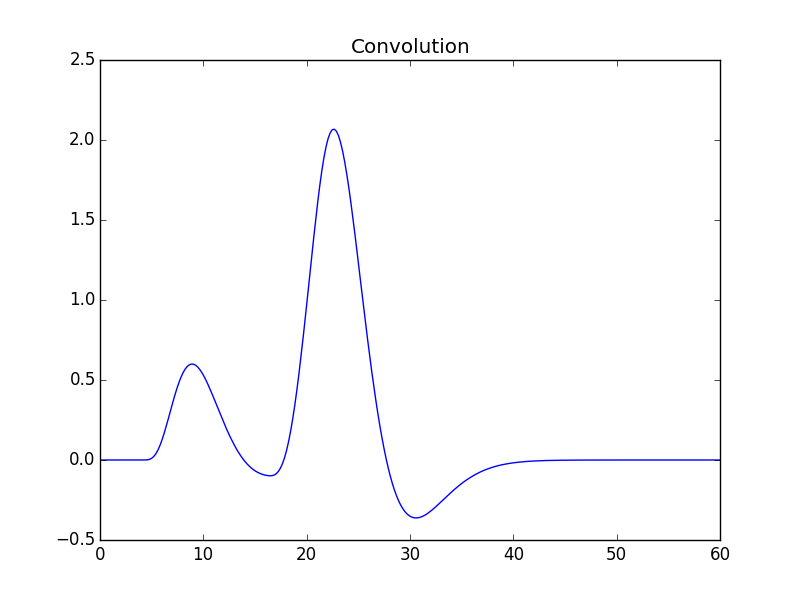
\includegraphics[width=.5\linewidth]{../images/initial_convolved.png}
	\caption{Convolution of $f$ and $g'$.}
	\label{fig:convolve1}
\end{figure}

\subsection{Approach to our Specific Problem}

\subsubsection{Returning to Our fMRI Data}

We can now apply this discrete approach to convolution between $f$ and $g'$ 
to our data. The $f$ is actually a common representation of the hemodynamic 
response, and the $g'$ is a good representation of the stimuli from an 
event-related trial \cite{brett2015course}. 

\subsubsection{Naive Approach (using \texttt{np.convolve})}

A \texttt{numpy} function \texttt{np.convolve}, which takes advantage of 
fast Fourier transforms for efficiency (it boils down to fewer computations 
using roots of unity) is commonly used to do discrete convolution. A naive 
approach for convolving two functions would use this function directly, but
\texttt{np.convolve} assumes that the intervals between stimuli mirror the 
desired intervals between prediction intervals. As such, we should not naively 
apply \texttt{np.convolve} to our data (though we do for a base model). 
Even so, exploring this naive approach for convolving the hemodynamic response 
gives an idea about what not to do, and sets a higher bar for accuracy.

\subsubsection{Needed Improvements: Moving beyond naive \texttt{np.convolve}}

Our data fails to meet the assumption that the intervals are equidistant, 
which is required to naively apply \texttt{np.convolve}. Especially in our 
case, there was not an simple fix, such as performing some basic rounding in 
order to then correctly utilize \texttt{np.convolve}. All the following 
approaches improve on the basic \texttt{np.convolve} approach's accuracy, but 
ultimately circle back to incorporating \texttt{np.convolve} to improve the 
speed of the convolution.

Our condition file (\texttt{cond1}) lists stimulus times for when the 
individual pumped the balloon but did not pop it. For subject 001, the 
first 10 data points are as follows [Figure \ref{table:cond1}]:

\vspace{5mm}

\begin{figure}[ht]
\begin{center}
\begin{tabular}{|cccccccccc|}
  \hline
0.0671 &
2.1251 &
3.7681 &
5.6601 &
7.8673 &
9.3443 &
19.7831 &
22.0402 &
23.5837 &
25.1434 \\
 \hline

  \end{tabular}
   \caption{First 10 values for Sub 001, condition 1.}
  \label{table:cond1}
\end{center}
\end{figure}
 
Clearly, this short time series does not align with idealized scans that 
start at $t=0$ and occur every two seconds apart. As such, we had to go back 
to the drawing board to try to reproduce our expected hemodynamic response for 
the entire time course.


\subsection{Summary of Approaches}
Our first approach attempts to correctly match the theory underlying our data. 
Our second approach tries to utilize \texttt{np.convolve} by expanding the 
grid of desired results (thanks to advice from  Matthew Brett, Jean-Baptiste 
Poline, and Jarrod Millman).


\subsubsection{Initial Correction to Represent Theoretical Idea}
To account for our data's lack of any easily identifiable grid structure 
between when a stimulus was recorded and when our scans occurred (on the 
order of every 2 seconds), we went back to the theory of convolution and 
implemented code to recreate equation \ref{eq:math_discrete_final} directly. 
To do so, we also had to create a function that works with all discrete points 
of $f$, the stimulus response as potential starts of the hemodynamic response, 
multiplied by the actual value of $f$, as seen in equation 
\ref{eq:code_convolve}:

\begin{equation} \label{eq:code_convolve}
r(t)= \sum_{i=1}^n g'_{i} f(t-t_i)
\end{equation}

where $g'_{i}$ is the value of $g'$ at $t_i$ (allowing for zeros and varying 
non-zero values of $g'$).


\subsubsection{Matrix Multiplication}
Equation \ref{eq:code_convolve}, reproduced below

$$r(t)= \sum_{i=1}^n g'_{i} f(t-t_i)$$

can be rewritten as a matrix multiplication problem and can be seen below:

\begin{equation} \label{eq:matrix_code_convolve}
r(t)=  g^*(t)^T f^*(t)
\end{equation}

where $g^*$ is a vectorized function of $g'$ of $t$ as a scalar output and 
$f^*$ is the vector of $f$ values (irrespective of location, as the $t^*$ 
takes that into account). This is a useful representation, since matrix 
multiplication is faster for Python's numpy arrays. 


\subsubsection{Using FFT with \texttt{np.convolve}}
The ``theoretical'' solution lacked computation efficiency (despite 
considerable speed improvements from matrix multiplication), so we also 
approached the problem by creating a denser grid between each scan (two seconds 
apart). Then we rounded the actual times of the stimulus to meet this more 
finely scaled grid. This allowed us to utilize \texttt{np.convolve} with its 
faster, FFT-based algorithms, before reducing back down to our two-second 
grid. 


\subsection{Example}

Now that we have discussed the theory and possible implementations 
for convolving event-related stimulation, we will look at a basic example from 
our data. In doing so, we examine the trade-offs between theoretical accuracy 
and computational efficiency. We will consider just subject 001's condition 
files. 


\begin{figure}[ht]
\centering
	\begin{minipage}[b]{0.45\linewidth}
		\centering
		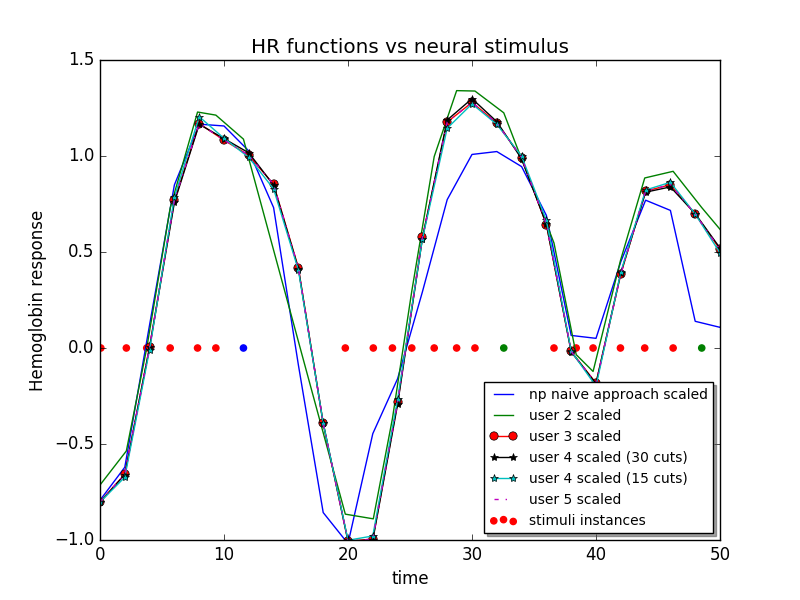
\includegraphics[width=.8\linewidth]{../images/convolution_vs_neural_stimulus}
		% needs to be from the event_related_HRF_script2.py 
		\caption{\scriptsize{Different convolution functions vs. the Neural stimulus}}
		\label{fig:convolution}

	\end{minipage}
\quad
	\begin{minipage}[b]{0.45\linewidth}
		\centering
		\begin{tabular}{|l | c|}
		\hline
		name in graph       & Speed per loop \\
		\hline
		np naive approach & 14.4 $\mu$s  \\
		user 2     		    & 972 ms  \\
		user 3     		    & 1.15 s    \\
		user 4 (15 cuts)      & 98.3 ms \\
		user 4 (30 cuts)      & 185 ms  \\
		user 5     	 	    & 110 ms   \\
		\hline
		\end{tabular}
		\vspace{5mm}
		\caption{\scriptsize{Speed to create HRF predictions for Subject 001, 
		all conditions}}
		\label{table:convolution}
	\end{minipage}
\end{figure}

The first method in the table ``np naive approach'' method blindly plugs 
our data into the \texttt{np.convolve} function and is provided to showcase 
potential speed. The ``user 2'' method  was the first approach to match the 
theory, though it matches the stimulation times instead of the scan times. 
The ``user 3'' method is the most theoretically sound model (and is our 
standard for accuracy). The ``user 5'' model  is our matrix version of  
``user 3'' and has the same accuracy, but is observably faster. The 
``user 4'' methods involve the grid cut usage of \texttt{np.convolve}
with notations for the number of slices between each scan. We concluded that 
"user 4 (15 cuts)" was the best approach since it gives us speed and very 
close accuracy to the golden standard --- "user 3".






%While this final method does lose some accuracy compared to the more 
%theoretically rigorous approach, the trade-off brings considerable gains in 
%computational efficiency. 


%Needed references:
%Brett, Matthew and Poline, J-B  (2013). Convolution. Retrieved from 
% http://practical-neuroimaging.github.io/on_convolution.html

% Weissten, Eric W. ``Convolution''. From MathWorld - A Wolfram Web  Resource. 
% Retrieved from htt://mathworld.wolfram.com/Convolution.html



\section{Time Series Analysis} \label{app_time}

\documentclass[11pt]{article}

\usepackage[margin=0.75in]{geometry}
\usepackage{indentfirst}
\usepackage{graphicx}
\bibliographystyle{siam}

\title{Appendix: Time Series Analysis}
\author{
  Chen, Kent\\
  \texttt{kentschen}
  \and
  Lee, Rachel\\
  \texttt{reychil}
  \and
  LeRoy, Benjamin\\
  \texttt{benjaminleroy}
  \and
  Liang, Jane\\
  \texttt{janewliang}
  \and
  Udagawa, Hiroto\\
  \texttt{hiroto-udagawa}
}

\begin{document}
\maketitle

\par \indent Cohen's paper \cite{CohenSelfControl} discusses analyzing the 
data with time series using FILM (FMRIBs Improved Linear Model). While we are 
not familiar with the FILM method, we did try modeling individual voxels in 
the framework of an autoregressive integrated moving average (ARIMA) process. 
We focused only on a single voxel from the first subject, but the method 
could easily be extended to additional or aggregate voxels. Let $\{Y_t\}$ be 
a single volume's value at time $t$ and assume that the $d$th difference 
$W_t = \nabla^d Y_t$ is weakly stationary, defined to be when $W_t$ has a 
constant mean function and autocovariance dependent only on lag $k$ and not 
time $t$. Then we can try to model $W_t$ as a linear combination of $p$ 
autoregressive terms (or the number of most recent values to include) and $q$ 
moving average terms (the number of lags to include for the white noise error 
terms): 
$$W_t = \phi_1 W_{t-1} + \phi_2 W_{t-2} + ... + \phi_p W_{t-p} + e_t - 
\theta_1 e_{t-1} - \theta_2 e_{t-2} - ... - \theta_q e_{t-q}.$$

\par White noise is defined as a sequence of independent, identically 
distributed random variables. In order to fit an ARIMA process, the three 
orders $p$, $d$, and $q$ must be first be specified, and the the associated 
coefficients estimated. We used a combination of visual inspection and 
quantitative methods to specify the ARIMA orders, and then used the maximum 
likelihood method to estimate parameters. 

\par Having specified the order for $d$, we turned to the problem of 
specifying $p$ and $q$. We used a combination of visually inspecting the 
autocorrelation and partial autocorrelation plots of the first difference, 
and looking at the Akaike information criteria (AIC) and Bayesian information 
criteria (BIC) computed from a grid of possible models. The latter method 
suggested specifying $p=1$ and $q=1$ (based on either the AIC or the BIC), 
which was also supported by the visual inspections. 

\par We estimated the parameters for an ARIMA(1,1,1) model using the exact 
maximum likelihood estimator via Kalman filter. The residuals appear to be 
normally distributed, and its autocorrelation and partial autocorrelation 
plots also do not raise any red flags. Furthermore, when visually comparing 
the fitted time series to the true observed data, the ARIMA process seems to 
approximate the observed data much better than any of the linear regression 
models. However, since specifying the correct ARIMA process orders and 
estimating the associated parameters must be done separately by hand for 
each individual voxel of interest, we decided to eliminate this direction 
of analysis from our main pipeline. 

\par Had we decided to continue pursuing time series analysis, we may have 
tried to forecast future observations based on previous ones. As an example, 
we modeled an ARIMA(1,1,1) process based on the first half of the 
observations for a single voxel. This process was then used to forecast the 
second half of the observations. A comparison between the true observations 
and the forecasted predictions is shown in [Figure \ref{fig:ts-preds}]. 
While the forecasted observations look reasonable for approximating the true 
values, more quantitative metrics for assessing performance need to be 
implemented. 

\begin{figure}[ht]
\centering
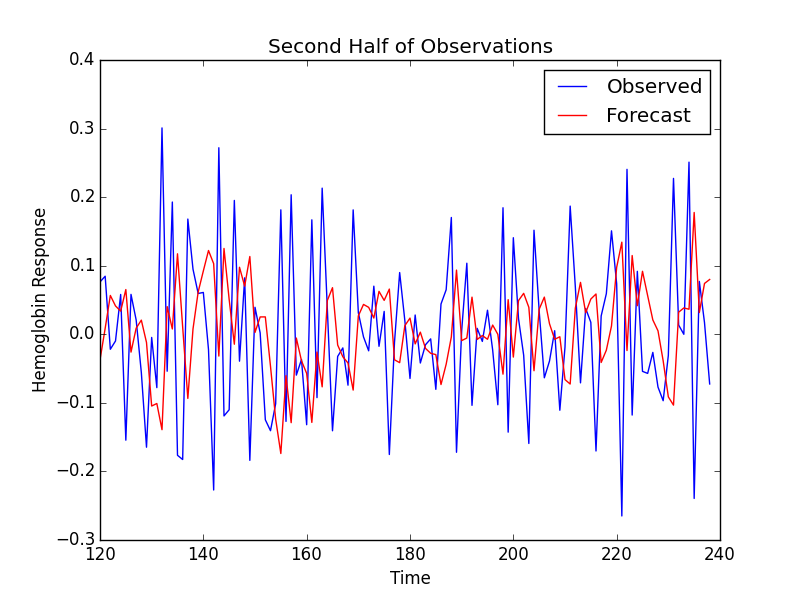
\includegraphics[scale=0.5]{images/ts-preds.png}
\caption{Forecasting the second half of observations based on the first 
half.}
\label{fig:ts-preds}
\end{figure}

\par One such procedure for assessing performance would be to design a 
permutation test. A null voxel time course could be simulated from by 
performing a Fourier transform on the observed time course, permuting the 
phase, and then transforming back to the original space. That way, the 
simulated time course has the same autocovariance as the observed time 
course, but random signal (as under the null case). Other considerations 
for modeling voxels as time series include exploring efficient and 
reasonable techniques for comparing multiple voxels both within and across 
subjects. 

\bibliography{project}

\end{document}



		



\bibliography{project}
\end{document}
